\documentclass[fleqn,usenatbib]{mnras}

\usepackage{newtxtext,newtxmath}
\usepackage[T1]{fontenc}
\DeclareRobustCommand{\VAN}[3]{#2}
\let\VANthebibliography\thebibliography
\def\thebibliography{\DeclareRobustCommand{\VAN}[3]{##3}\VANthebibliography}
\usepackage{graphicx}	% Including figure files
\usepackage{pict2e}
\usepackage{amsmath}	% Advanced maths commands
%\usepackage{amssymb}	% Extra maths symbols

%%%%%%%%%%%%%%%%%%%%%%%%%%%%%%%%%%%%%%%%%%%%%%%%%%

%%%%% AUTHORS - PLACE YOUR OWN COMMANDS HERE %%%%%

% Please keep new commands to a minimum, and use \newcommand not \def to avoid
% overwriting existing commands. Example:
%\newcommand{\pcm}{\,cm$^{-2}$}	% per cm-squared

%%%%%%%%%%%%%%%%%%%%%%%%%%%%%%%%%%%%%%%%%%%%%%%%%%

%%%%%%%%%%%%%%%%%%% TITLE PAGE %%%%%%%%%%%%%%%%%%%

% Title of the paper, and the short title which is used in the headers.
% Keep the title short and informative.
\title[Artificial Pulsar]{Tuning Low Frequency Pulsar Searching with an  Artificial Pulsar Device}

\author[J.-H. Gu et al.]{
Junhua Gu$^{1}$\thanks{E-mail: jhgu@nao.cas.cn} et al.
\\
% List of institutions
$^{1}$National Astronomical Observatories, Chinese Academy of Sciences, 20A Datun Road, Beijing, China
}
% These dates will be filled out by the publisher
\date{Accepted XXX. Received YYY; in original form ZZZ}

% Enter the current year, for the copyright statements etc.
\pubyear{2021}

% Don't change these lines
\begin{document}
\label{firstpage}
\pagerange{\pageref{firstpage}--\pageref{lastpage}}
\maketitle

% Abstract of the paper
\begin{abstract}
Abstract
\end{abstract}

% Select between one and six entries from the list of approved keywords.
% Don't make up new ones.
\begin{keywords}
keyword1 -- keyword2 -- keyword3
\end{keywords}

\section{Introduction}
\citet{2017AAS...22915516P}, \citet{2011AAS...21723406S}

\section{Artificial Pulsar Device}
The artificial pulsar device (APD hereafter) is a device that is able to emit simulated pulsar signal within some certain bandpass.
We design it to be able to simulate the dispersion effect and arbitrary pulse profile of a pulsar.
Our implementation of APD is composed of three modules: 1) a high performance workstation that is responsible of computing the pulsar signal online, 2) a software-defined radio (SDR) transmitter that accepts commands and data stream from the workstation and convert it to voltage signal, which is then fed into 3) a radio frequency front-end. 
The radio frequency front-end is further composed of a radio frequency power amplifier (PA hereafter) and an antenna that is used to broadcast the actual signal.

\begin{figure}
    \centering
    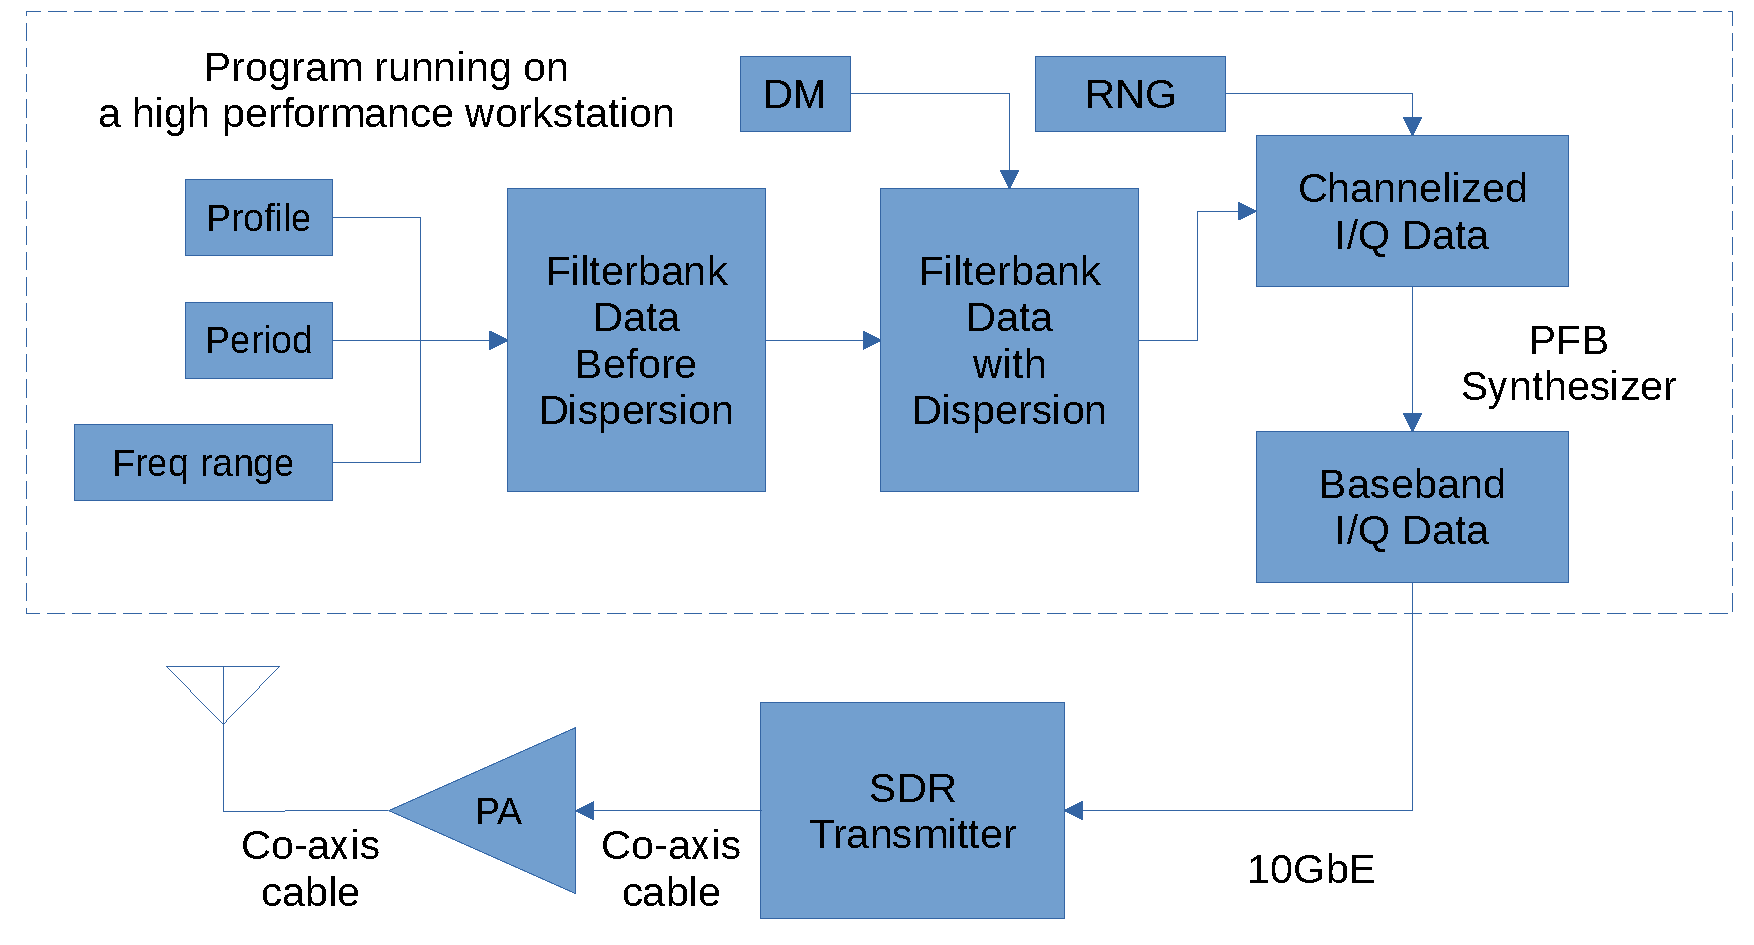
\includegraphics[width=0.95\columnwidth]{flow_chart.pdf}
    \caption{The flow chart of emitting the simulated pulsar signal.
    }
    \label{fig:flow_chart}
\end{figure}


The APD can be placed near the low-frequency pulsar observation device (LFPOD hereafter). 
Though possible, it is not necessary for the emitting antenna to be placed inside the range of the primary beam LFPOD.
The power of the emitted signal can be amplified to a high enough level so that when the signal is received by the LFPOD from its side lobes it approximates the power level of a natural pulsar.

In this section, we describe the algorithms and steps that are used to generate the radio frequency signal, which is later used to tune LFPODs.

\subsection{Important Approximations that We Make}
The purpose of this work is to present a method of tuning the search of pulsars in low frequency radio band, which is composed of signal receiving/recording and signal detection.
Dedispersion is an important step in the signal detection stage.
According to e.g., \citet{2012hpa..book.....L}, it is possible to perform either coherent dedispersion or incoherent dedispersion. The former works on raw baseband data and the latter works on channelized filterbank data. 
The main different between these two category of dedispersion methods is whether phase information is kept in the input data.
In order to enable the generated signal suitable to both category of dedispersion methods, we have to ensure that the phase information is treated with caution.
Considering that fact that the dispersion caused by ISM can cause delays of different frequencies in low frequency band to reach at most $10^2$ s time scale, computing the dispersed pulsar signal online without necessary approximation is infeasible.

We make following approximation when generating the artificial pulsar signal: the pulsar signal (not only the amplitude profile, but also the signal phase) repeats with a period of $n\tau$, where $\tau$ is the period of the pulsar, $n$ is an integer. The value of $n$ is chosen so that it is affordable by the computation resource of the workstation that we use to generate the signal and large enough to ensure good enough statistics in folding. 
With above approximation the frequency components contained in the signal become discrete so that the phase delays of all the frequency components can be computed precisely.

In practice, we choose the value of $n\tau$ around $1$ s.
As the signal can be computed offline, this value can reach several seconds to dozens of seconds.
If incoherent dedispersion method is used, it is also possible to update the repeating signal samples every tens of seconds (this time interval is determined by computing performance), for the phase information is not important. 


\subsection{Computing Artificial Pulsar Signal}
\subsubsection{Generating baseband I/Q samples}
The pulse amplitude profile $f(\theta)$, where $\theta$ is the pulse phase should meet following constraint
\begin{gather}
    f(\theta+1)=f(\theta).
\end{gather}
In following sections we utilize a Gaussian function with a pulse width parameter $w$ to describe the profile:
\begin{gather}
    f(\theta)=\left \{
    \begin{array}{rl}
        f(\theta-1) &\theta \geq 0.5\\
         \exp(-\frac{\theta^2}{2w^2}) & \theta\in[-0.5, 0.5) \\
        f(\theta+1) &\theta < -0.5\\
    \end{array}
    \right ..
\end{gather}
Assuming a frequency range of $[\nu_{\min}, \nu_{\max}]$, the sampling interval $dt$ is also fixed as $dt=1/B$, where $B=\nu_{\max}-\nu_{\min}$.
Thus the baseband I/Q sample series is generated as 
\begin{gather}
    y_j=f(\frac{j\times dt}{\tau})\frac{x^{\rm re}_j+x^{\rm im}_ji}{2}, j=1..\left \lfloor\frac{n\tau}{dt} \right\rfloor
\end{gather}
where each $x^{\rm re}$'s and $x^{\rm im}$'s independently follows a standard normal distribution. 


 \subsubsection{Applying the dispersion effect}
  Applying the ISM dispersion effect is simply an inverse operation of coherent dedispersion with some slight differences.
  According to e.g., \citet{2012hpa..book.....L}, we calculate the dispersed baseband I/Q sample series as
  \begin{gather}
      \mathbf{y}^d={\rm IDFT}(\mathbf{Y}^d)
  \end{gather}
  \begin{gather}
      Y_j^d={\rm DFT}(\mathbf{y})_j\exp(2\pi i \nu_j\Delta t(\nu_j)),
  \end{gather}
  where ${\rm DFT}$ and ${\rm IDFT}$ denote the forward and backward discrete Fourier transform, respectively, $\mathbf{y}$ is a vector with each of its element to be $y_j$, $\mathbf{Y}$ is a vector with each of its element to be $\mathbf{Y}_j$, $\nu_j$ is the frequency corresponding to the $j$-th frequency channel, and the delay cause by the dispersion is calculated as 
  \begin{gather}
     \Delta t(\nu)\simeq 4.15\times 10^6~{\rm ms}~\left(\frac{{\rm MHz}}{\nu}\right)^2\frac{\rm DM}{\rm pc~cm^{-3}},
 \end{gather}
 according to e.g., \citet{2012hpa..book.....L}.
 
 We present two examples of the time domain I/Q sampling data in Figure \ref{fig:iq_data} with ${\rm DM}=0$ pc~cm$^{-3}$ and DM=1 pc~cm$^{-3}$, respectively.
 The frequency range is set to be $100\sim 200$ MHz.
 Apparently the wide bandwidth and the low central frequency make the time domain data rather sensitive to the dispersion measure.
 ${\rm DM}=1$ is a rather small value of the dispersion measure among known pulsars.
 When trying to detect pulsars with larger dispersion measures in low frequency radio band, difficulties will appear caused by the the dispersion of ISM more seriously compared with higher radio bands.
 
 
\begin{figure*}
    \centering
    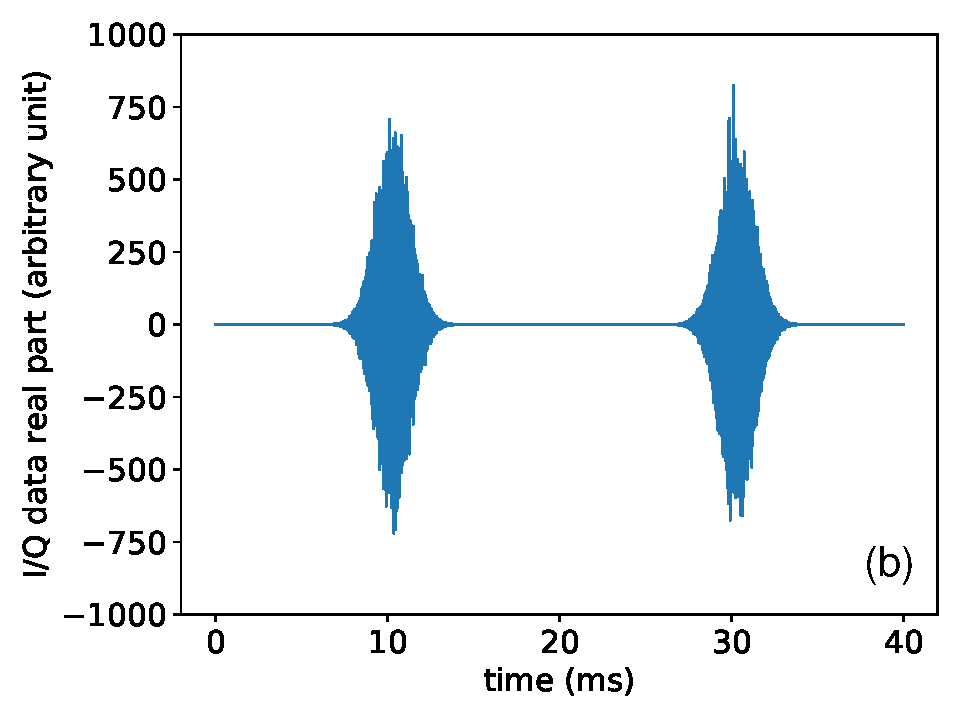
\includegraphics[width=0.95\columnwidth]{dm0_iq.pdf}
    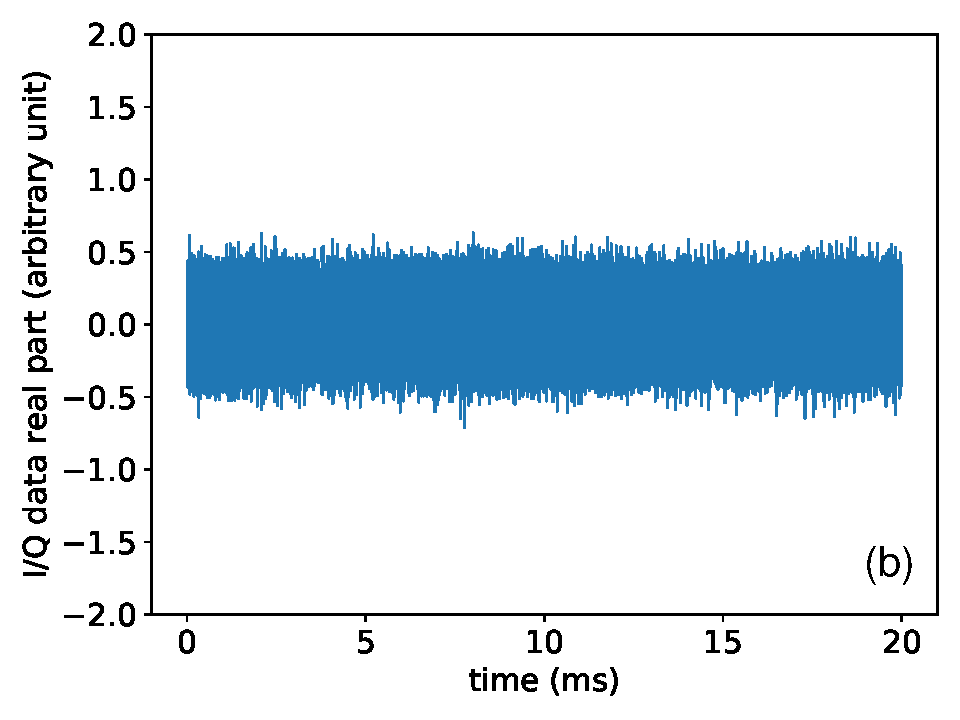
\includegraphics[width=0.95\columnwidth]{dm1_iq.pdf}
    \caption{The real part of the baseband I/Q data as a function of time. Two periods are shown here. The period is set to be 20 ms, in (a) the DM is set to be 10 pc cm$^{-3}$ and in (b), the DM is set to be 0 pc cm$^{-3}$ for the purpose of comparison.}
    \label{fig:iq_data}
\end{figure*}

We show the waterfall chart of above generated time domain I/Q data in Figure \ref{fig:fb} to inspect the frequency-dependent profile.
The waterfall chart is generated by feeding the time domain I/Q data stream into a polyphase filterbank.
Apparently for the ${\rm DM}=1$ pc~cm$^{-3}$ signal, lower frequency has larger delay, which agrees with properties of dispersion effect caused by ISM. 
This verifies the correctness of the signal we generated.

\begin{figure*}
    \centering
    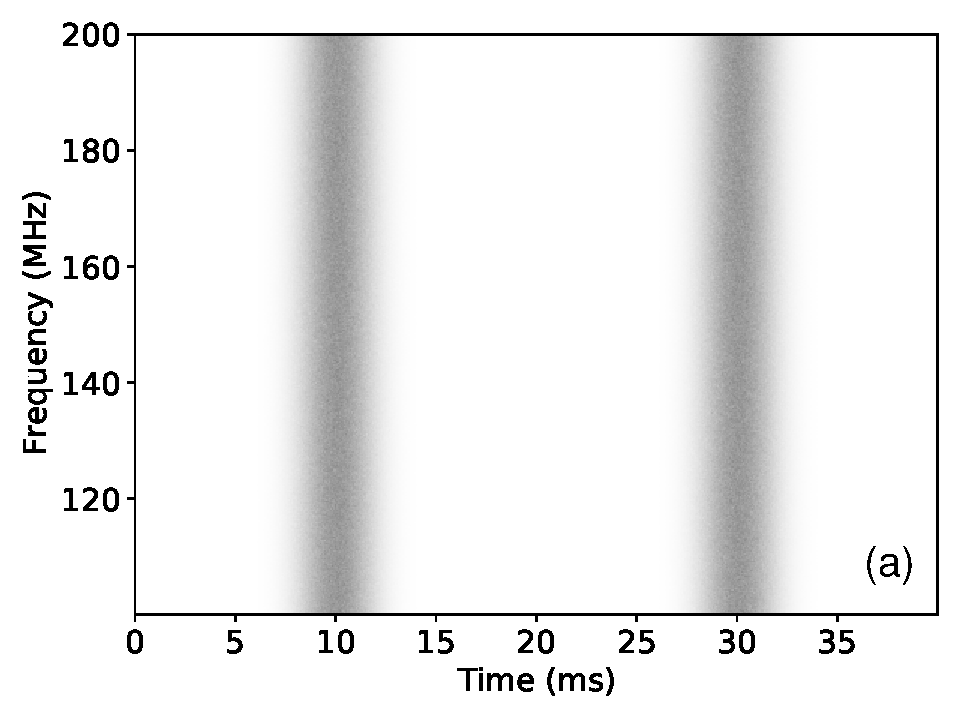
\includegraphics[width=0.9\columnwidth]{dm0_fb.pdf}
    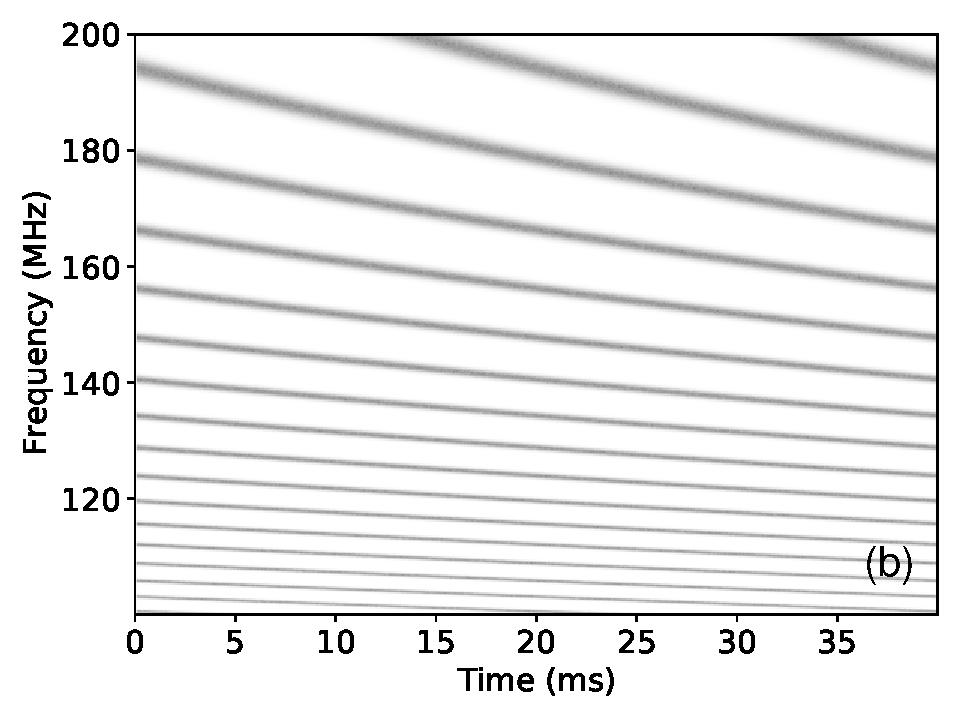
\includegraphics[width=0.9\columnwidth]{dm1_fb.pdf}
    \caption{Frequency dependent pulse profile with a $\rm DM=0$ pc cm$^{-3}$ (a) and $\rm DM=0$ pc cm$^{-3}$ (b) dispersion effect applied, respectively.}
    \label{fig:fb}
\end{figure*}


\subsection{Emitting Generated Signal}
The generated broadband I/Q data stream that has been dispersed is then fed into some radio frequency transmitter.
We use the software defined radio (SDR) transceiver \textit{USRP} X310\footnote{\url{https://kb.ettus.com/X300/X310}} to send the generated signal.
The maximum sample rate can reach 200 Msps, while we use a sample rate of 100 Msps corresponding to a bandwidth of $B=100$ MHz.
The corresponding frequency range is then $[\nu_c-B/2, \nu_c+B/2]$, where $\nu_c$ is the central frequency.
The SDR transceiver is connected to a high performance workstation through a 10Gb Ethernet fiber.
In this work we set the central frequency $\nu_c=150$ MHz, so that the frequency range is $100\sim 200$ MHz.


There are other choices of devices that can be used to transmit the generated signal, e.g.,  \textit{LimeSDR}\footnote{\url{https://limemicro.com/products/boards/limesdr}}, 
\textit{HackRF}\footnote{\url{https://greatscottgadgets.com/hackrf}}, and other general purpose digital-analog converter cards. 
The reason why choose \textit{USRP} X310 is its maximum instant bandwidth of 200 MHz, which enables us to emulate the conditions of most of current working low frequency radio telescopes.

The generated radio frequency signal is then amplified and broadcast through an antenna of the corresponding frequency range.
Before broadcasting and receive the signal through antennas, we use an oscilloscope to check the voltage signal at the output terminal of the SDR transceiver as are shown in \ref{fig:osc_trace}.

\begin{figure}
    \centering
    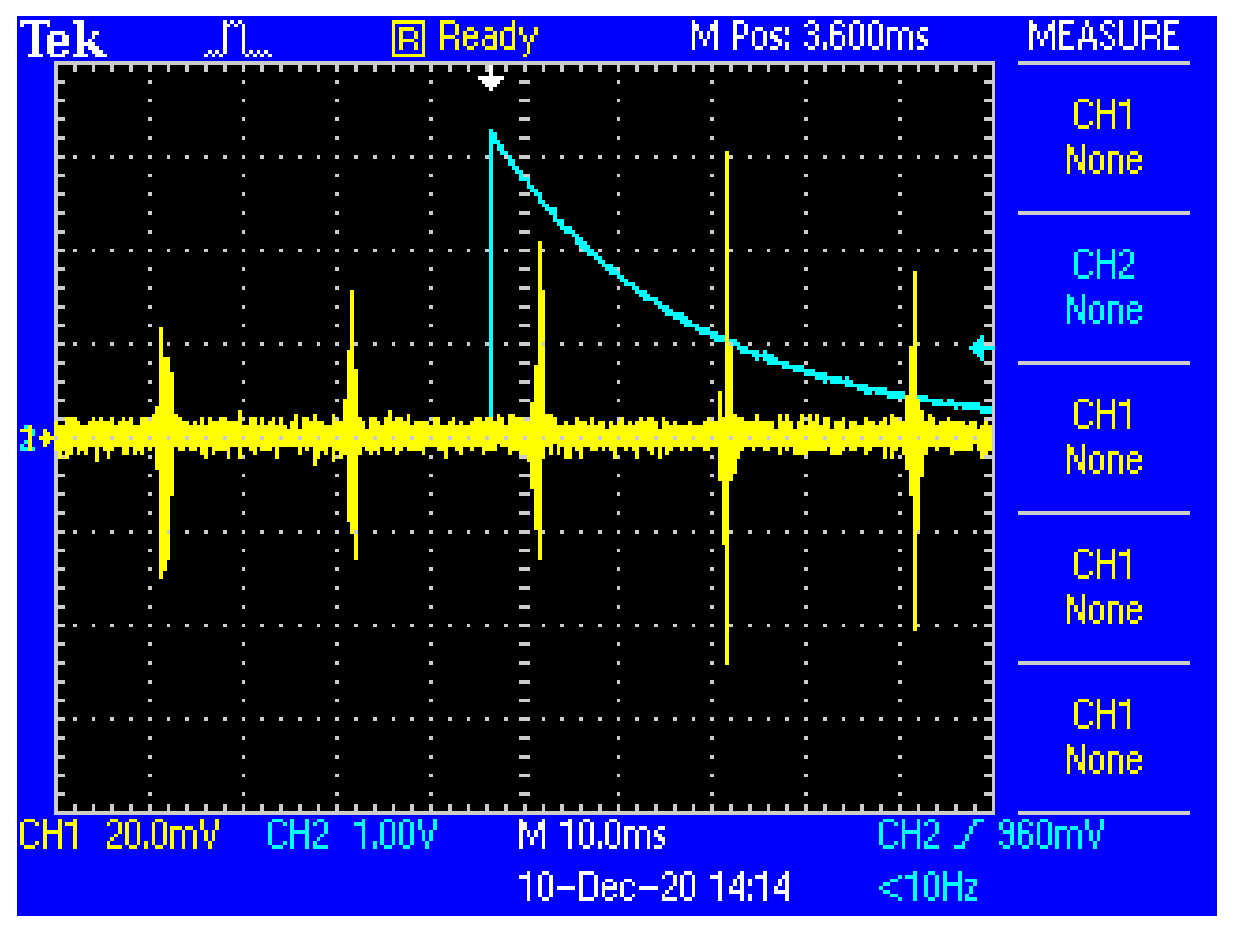
\includegraphics[width=0.45\columnwidth]{dm_0_trace.eps}
    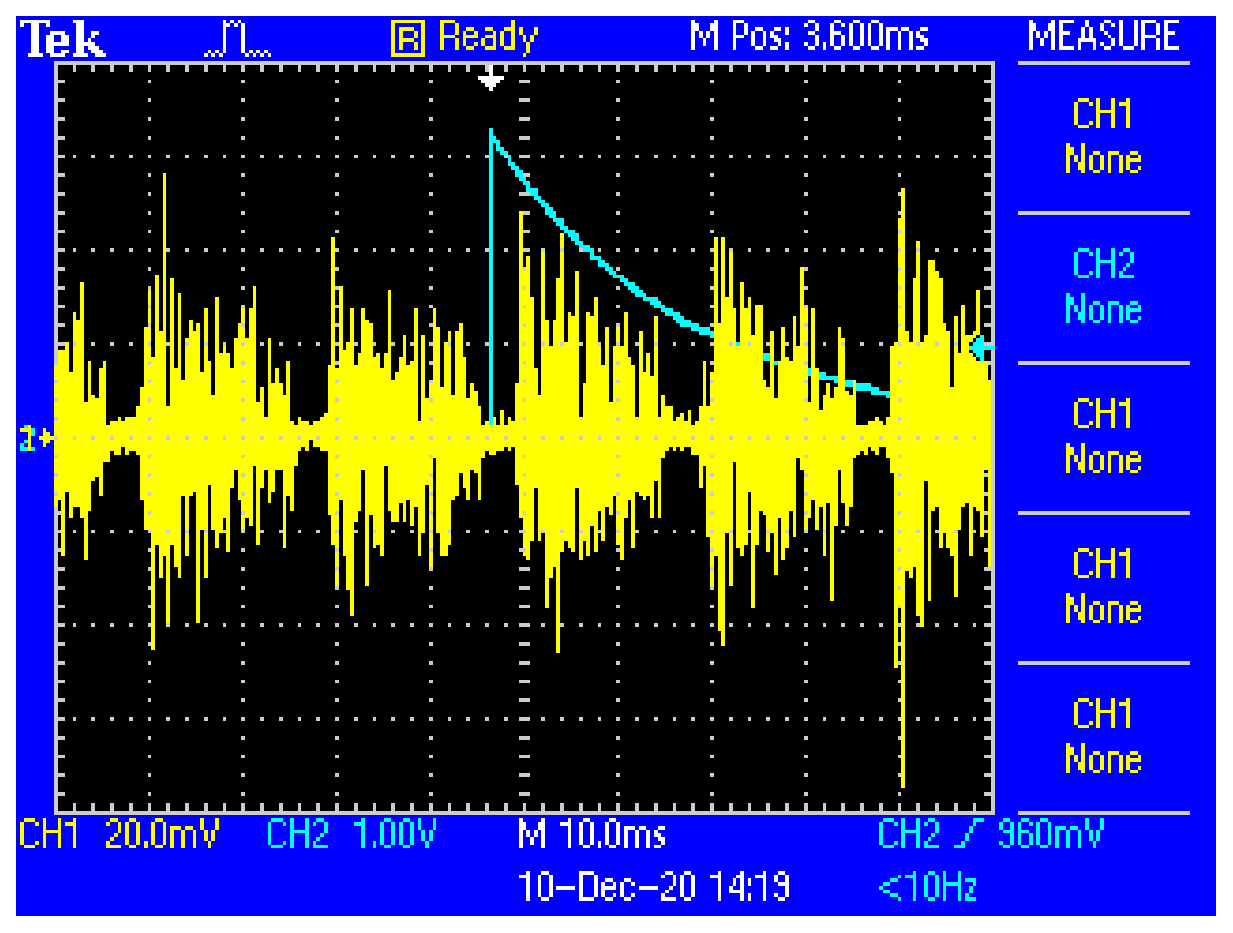
\includegraphics[width=0.45\columnwidth]{dm_0.05_trace.eps}
    \caption{The voltage signal trace (in yellow) observed with an oscilloscope at the output terminal of the SDR transceiver. The green lines are the PPS signal generated by the \textit{USRP} used to trigger the oscilloscope. The left and the right panel show signals with ${\rm DM}=0$ pc~cm$^{-3}$ and ${\rm DM}=0.05$ pc~cm$^{-3}$, respectively. The periods of both signals are set to be $20$ ms. Note that the lower limits of the frequency range of the generated signals are 100 MHz.}
    \label{fig:osc_trace}
\end{figure}

\section{Two Examples of Tuning}
We set up two experiments to demonstrate the process of tuning LFPODs to perform the pulsar signal detection. 
One of the experiment is using the SDR transceiver as a toy LFPOD.
Another experiment performed with the low frequency interferometer 21CMA.
For both experiment we follow the steps as
\begin{enumerate}
    \item Place the emitter (i.e., the \textit{USRP} X310 transceiver) close to the LFPOD;
    \item Set the emitter and the LFPOD to proper mode and start the data acquisition;
    \item After enough data is acquired and stored to disk, perform a pulsar search procedure to check whether the artificial pulsar signal can be recognized;
    \item If necessary, adjust the emitting setup.
\end{enumerate}

\subsection{HackRF---A Toy LFPOD}
\subsubsection{Setup of the experiment}
\textit{HackRF} is a low cost SDR transceiver with an operation frequency of 1 MHz$\sim$ 6 GHz.
The maximum sample rate is 20 MHz.
We place an \textit{HackRF} 1 m away from the emitter antenna to receive the signal.
As the distance is close enough, we do not use any external power amplifier either for the emitter and the receiver. 
The internal amplifier gains for the emitter and the receiver are set to 0 dB and 10 dB, respectively.
The sample rate of the receiver is set to 10 Msps, corresponding a bandwidth of 10 MHz and the central frequency is set to 150 MHz, which leads to a frequency range of $145\sim 155$ MHz.
The reason why we do not set the sample rate to its maximum allowed value is to prevent from packet dropping.

\subsubsection{Cases that we test}
We test two sets of artificial pulsar signal parameters, the periods of both are set to be 18 ms, and the DM's are respectively 10 pc~cm$^{-3}$ and 10 pc~cm$^{-3}$.

\subsubsection{Connecting the emitter and the receiver directly with a co-axis cable}
We connect the emitter and receiver directly with a co-axis cable to test whether the signal generating and data acquisition sub-modules work correctly.
We show the incoherently and coherently dedispersing and folding result in Figure \ref{fig:prepfold_direct_hackrf_dm100_18} and Figure \ref{fig:cddsp_direct_hackrf_dm100_18}, respectively.

\begin{figure}
    \centering
    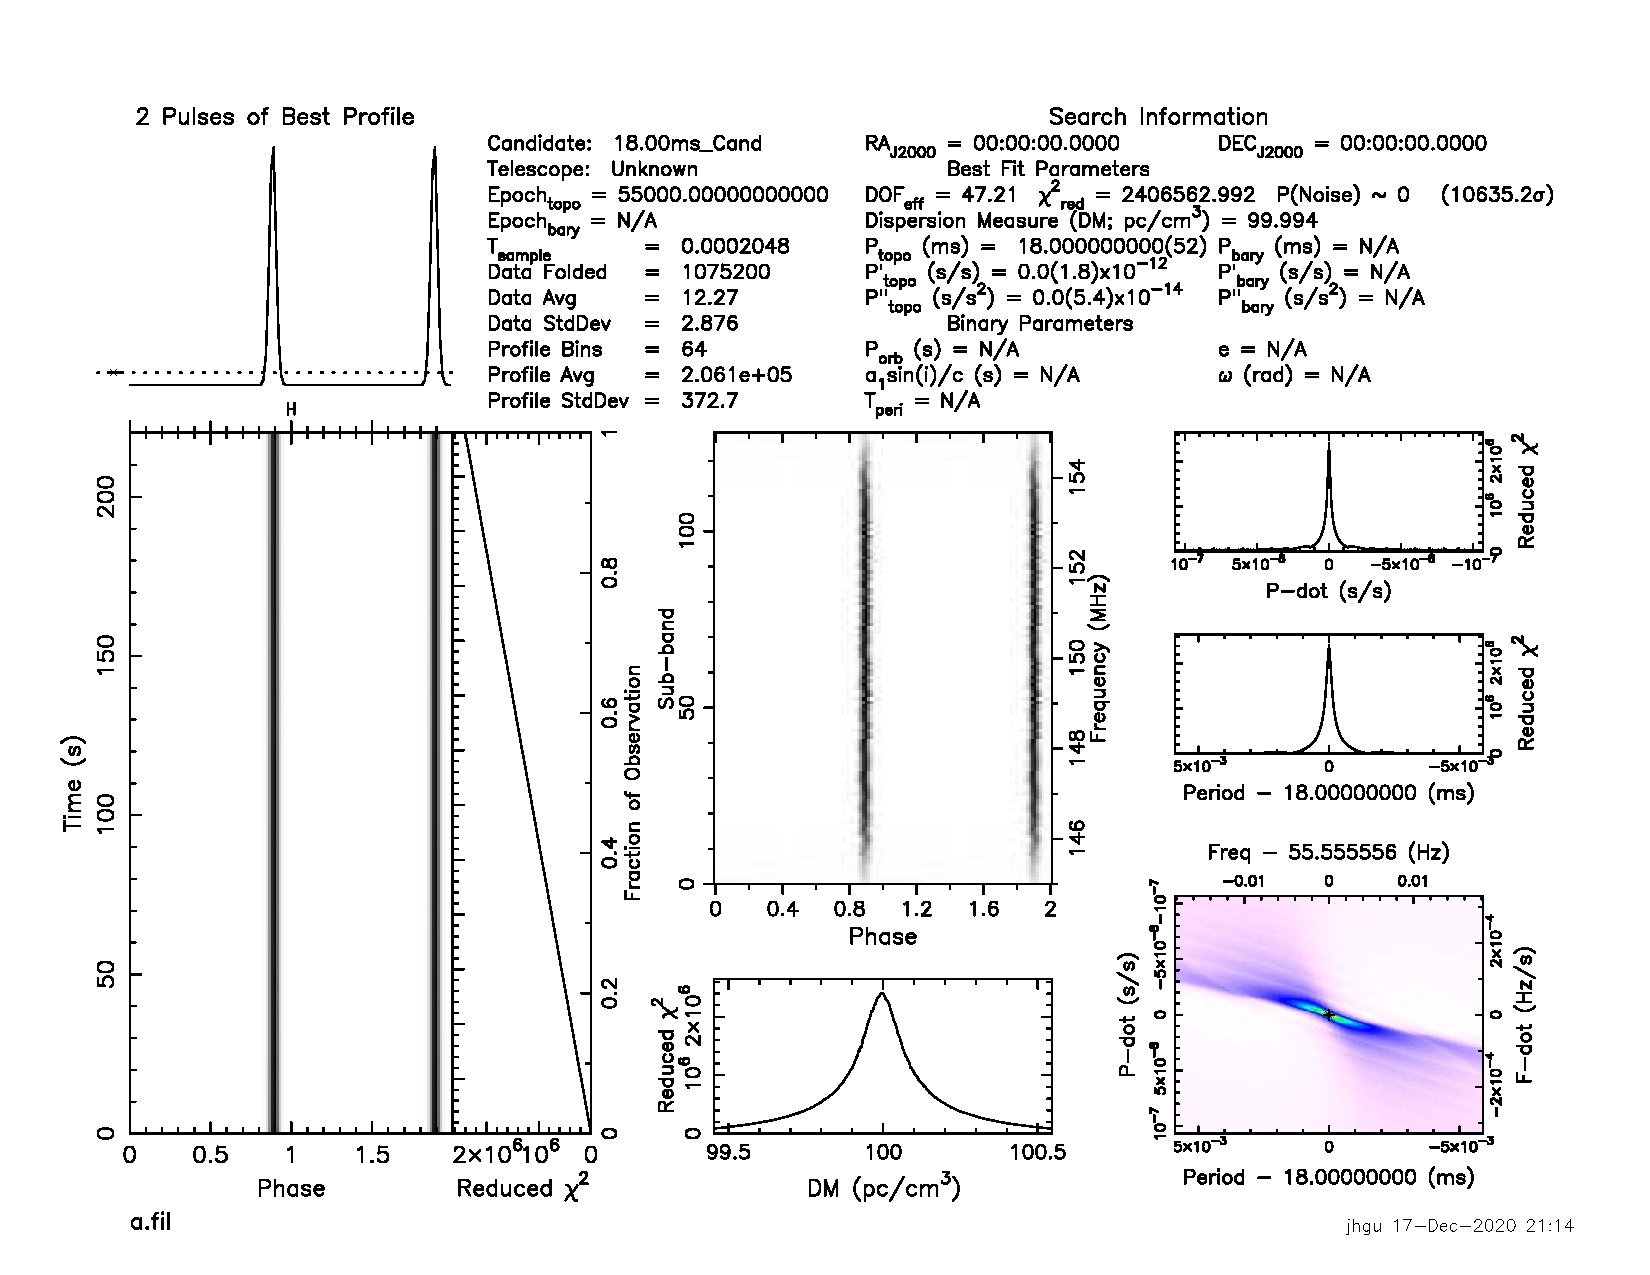
\includegraphics[width=\columnwidth]{prepfold_direct_hackrf_dm100_18.pdf}
    \caption{Incoherently dedispersing and folding result of the data acquired by \textit{HackRF} with the emitter and the receiver connected with a co-axis cable directly.}
    \label{fig:prepfold_direct_hackrf_dm100_18}
\end{figure}

\begin{figure}
    \centering
    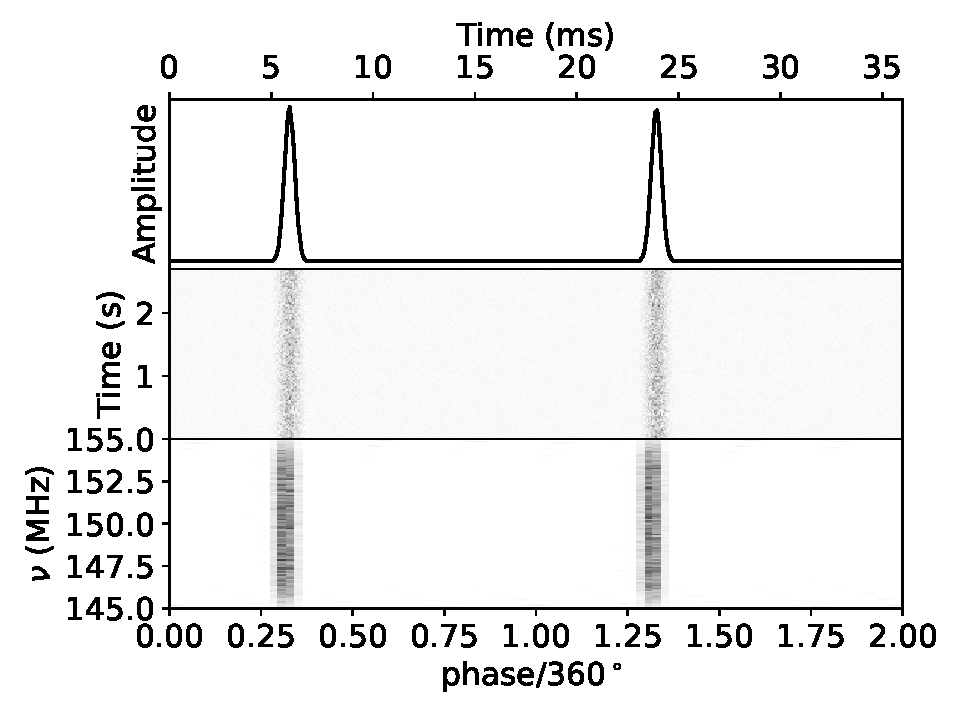
\includegraphics[width=\columnwidth]{cddsp_direct_hackrf_dm100_18.pdf}
    \caption{Coherently dedispersing and folding result of the data acquired by \textit{HackRF} with the emitter and the receiver connected with a co-axis cable directly.}
    \label{fig:cddsp_direct_hackrf_dm100_18}
\end{figure}

\subsubsection{Sending and receiving the signal through antennas}
Then we perform the data acquisition with the signal sent and received through antennas.



\section{Discussion}

\section{Conclusions}

\section*{Acknowledgements}


%%%%%%%%%%%%%%%%%%%%%%%%%%%%%%%%%%%%%%%%%%%%%%%%%%

\bibliographystyle{mnras}
\bibliography{ms}

%%%%%%%%%%%%%%%%%%%%%%%%%%%%%%%%%%%%%%%%%%%%%%%%%%


% Don't change these lines
\bsp	% typesetting comment
\label{lastpage}
\end{document}

% End of ms.tex
